\documentclass[a4paper,10pt]{article}
\usepackage{graphicx}
\graphicspath{{pics/}}
\begin{document}

\begin{figure}
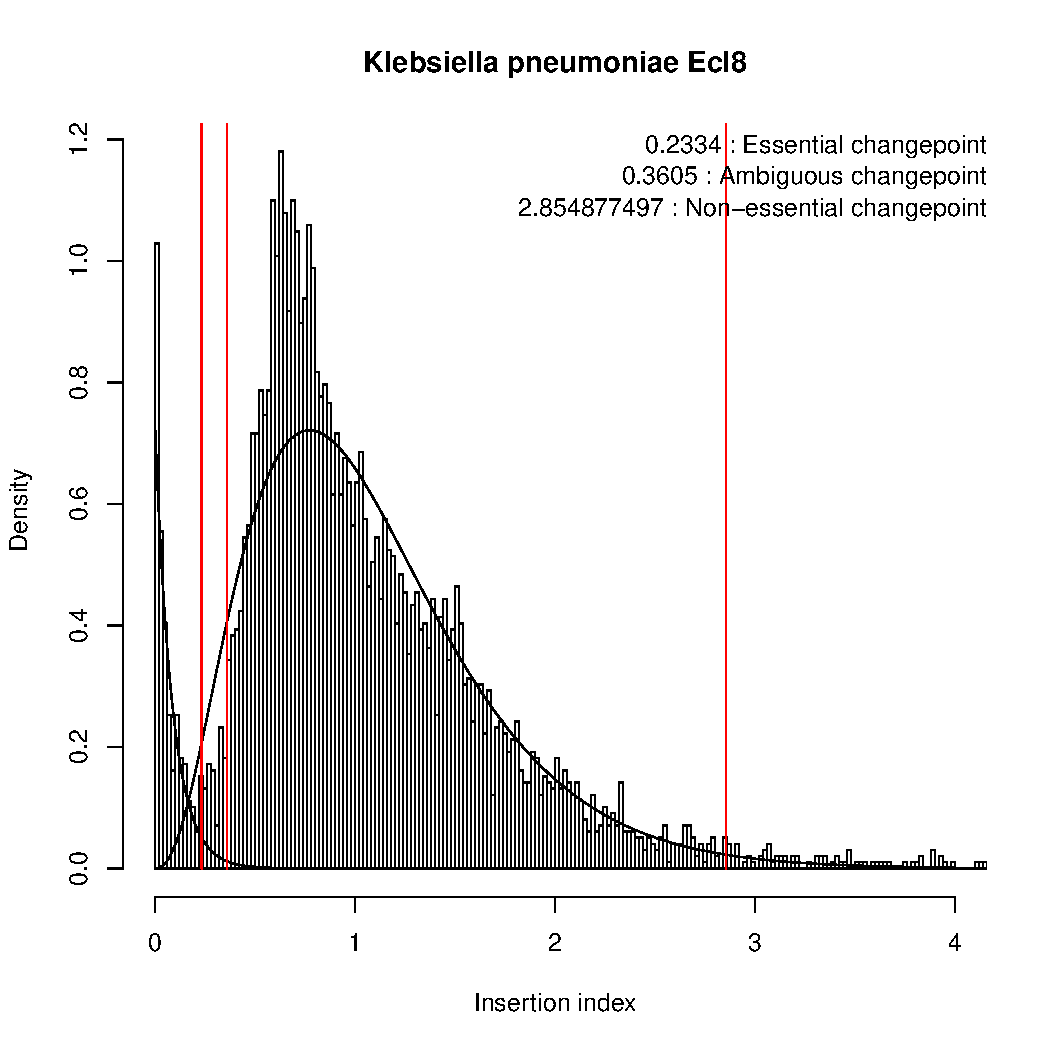
\includegraphics[scale=0.2, page=1]{mixtools.pdf}
\includegraphics[scale=0.2, page=2]{mixtools.pdf}
\includegraphics[scale=0.2, page=3]{mixtools.pdf}\\
\includegraphics[scale=0.2, page=4]{mixtools.pdf}
\includegraphics[scale=0.2, page=5]{mixtools.pdf}
\includegraphics[scale=0.2, page=6]{mixtools.pdf}\\
\includegraphics[scale=0.2, page=7]{mixtools.pdf}
\includegraphics[scale=0.2, page=8]{mixtools.pdf}
\includegraphics[scale=0.2, page=9]{mixtools.pdf}\\
\includegraphics[scale=0.2, page=10]{mixtools.pdf}
\includegraphics[scale=0.2, page=11]{mixtools.pdf}
\includegraphics[scale=0.2, page=12]{mixtools.pdf}
\caption{$ii=\frac{\frac{insertions(gene)}{length(gene)}}{\frac{insertions(genome)}{length(genome)}}$\newline
\textbf{Method:} gammamixEM \newline
\textbf{trimming:} 5 prime site: 5\%, 3 prime site: 10\%\newline
\textbf{plot manipulations:} Added 0.001 to all numbers, used Lars' shape and rate parameters \newline
\textbf{Number of essential genes:}\newline
Klebsiella pneumoniae Ecl8: 333\newline
Escherichia coli ETEC CS17: 563\newline
Enterobacter: 336\newline
Klebsiella pneumoniae RH201207: 329\newline
Escherichia coli ETEC H10407: 410\newline
Escherichia coli UPEC: 314\newline
Citrobacter: 319\newline
Salmonella enteritidis: 202\newline
Salmonella typhimurium SL1344: 423\newline
Salmonella typhimurium D23580: 309\newline
Salmonella typhimurium A130: 226\newline
Salmonella typhi: 266}
\end{figure}

\begin{figure}
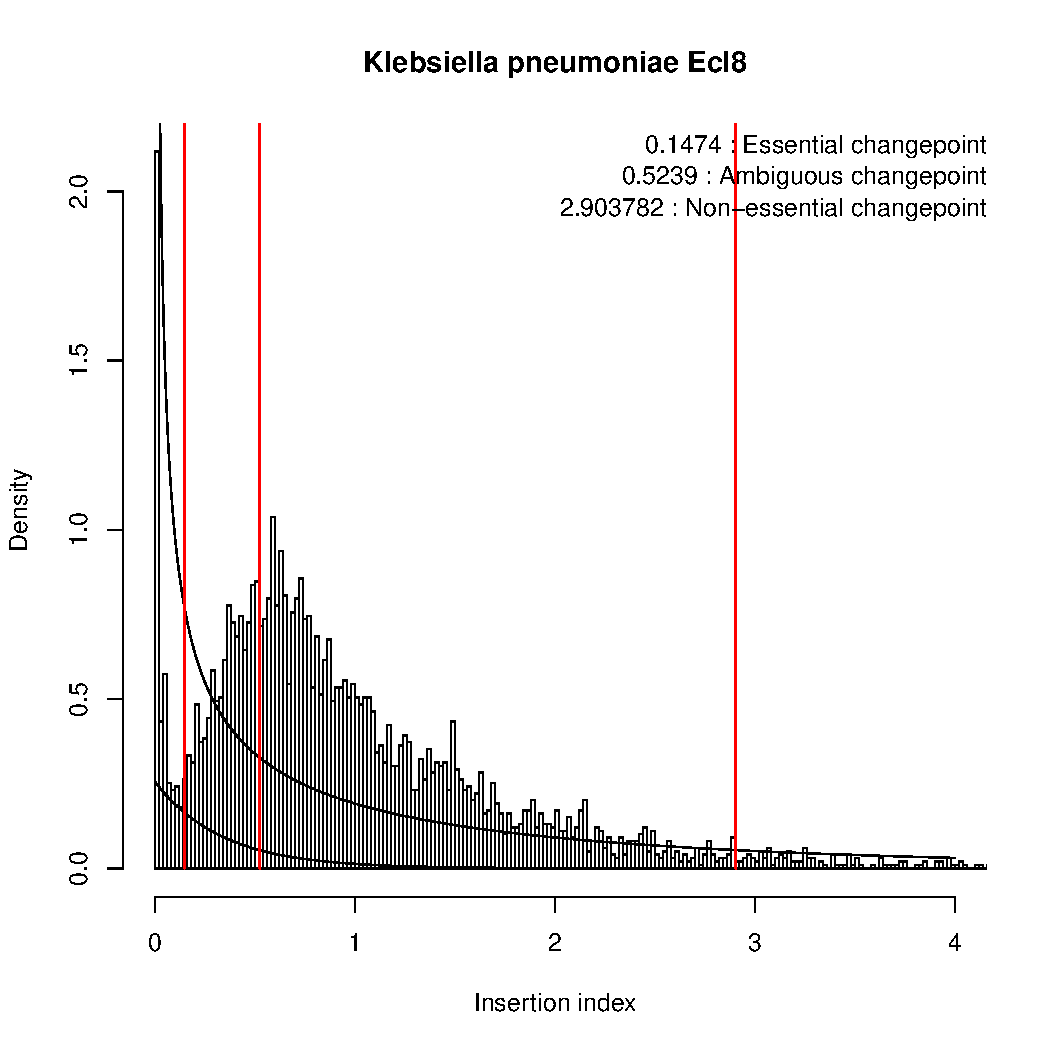
\includegraphics[scale=0.2, page=1]{mixtools-reads.pdf}
\includegraphics[scale=0.2, page=2]{mixtools-reads.pdf}
\includegraphics[scale=0.2, page=3]{mixtools-reads.pdf}\\
\includegraphics[scale=0.2, page=4]{mixtools-reads.pdf}
\includegraphics[scale=0.2, page=5]{mixtools-reads.pdf}
\includegraphics[scale=0.2, page=6]{mixtools-reads.pdf}\\
\includegraphics[scale=0.2, page=7]{mixtools-reads.pdf}
\includegraphics[scale=0.2, page=8]{mixtools-reads.pdf}
\includegraphics[scale=0.2, page=9]{mixtools-reads.pdf}\\
\includegraphics[scale=0.2, page=10]{mixtools-reads.pdf}
\includegraphics[scale=0.2, page=11]{mixtools-reads.pdf}
\includegraphics[scale=0.2, page=12]{mixtools-reads.pdf}
\caption{$ii=\frac{\frac{reads(gene)}{length(gene)}}{\frac{reads(genome)}{length(genome)}}$\newline
\textbf{Method:} gammamixEM \newline
\textbf{trimming:} 5 prime site: 5\%, 3 prime site: 10\%\newline
\textbf{plot manipulations:} Added 0.001 to all numbers \newline
\textbf{Number of essential genes:}\newline
Klebsiella pneumoniae Ecl8: 407 \newline
Escherichia coli ETEC CS17: 549 \newline
Enterobacter: 348 \newline
Klebsiella pneumoniae RH201207: 366 \newline
Escherichia coli ETEC H10407: 403 \newline
Escherichia coli UPEC: 369 \newline
Citrobacter: 343 \newline
Salmonella enteritidis: 269 \newline
Salmonella typhimurium SL1344: 353 \newline
Salmonella typhimurium D23580: 580 \newline
Salmonella typhimurium A130: 315 \newline
Salmonella typhi: 386}
\end{figure}

\begin{figure}
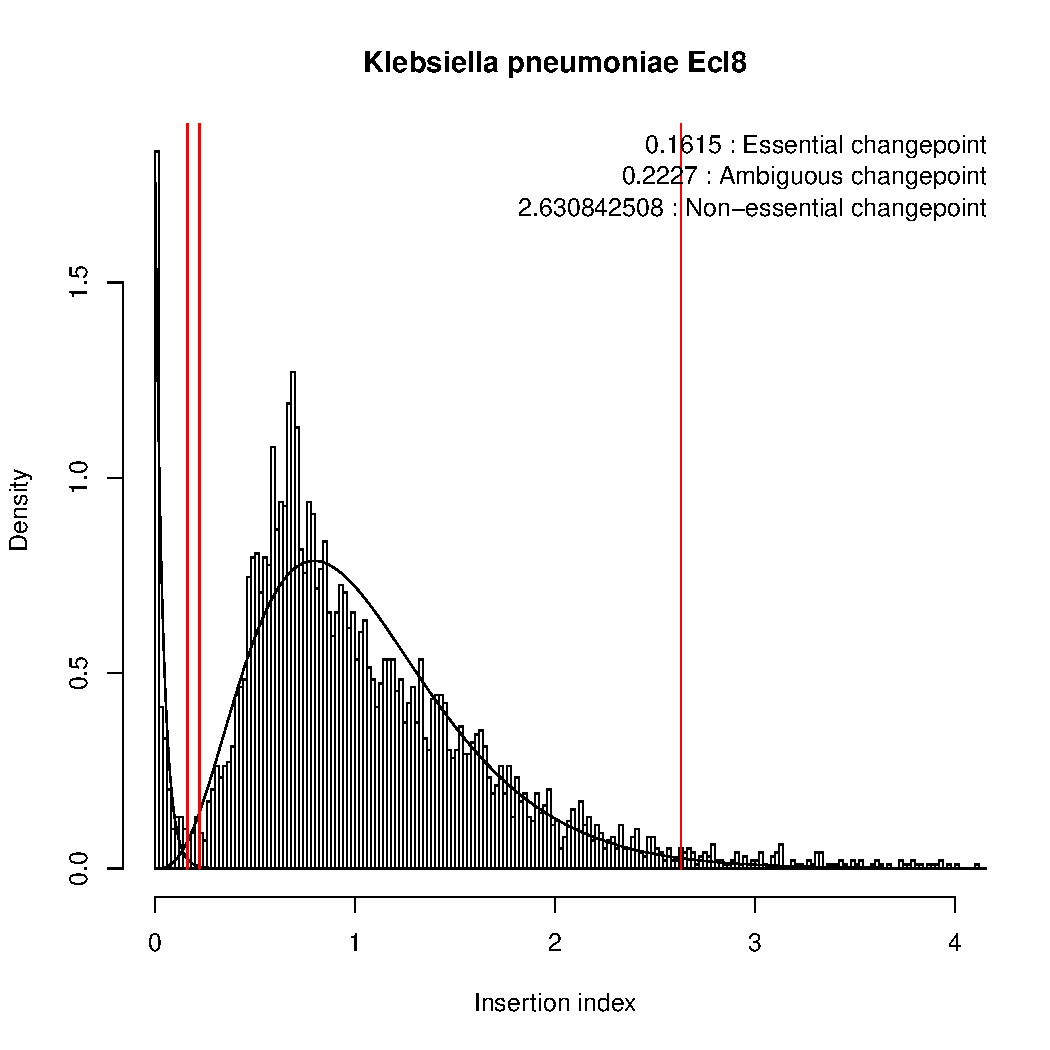
\includegraphics[scale=0.2, page=1]{lars.pdf}
\includegraphics[scale=0.2, page=2]{lars.pdf}
\includegraphics[scale=0.2, page=3]{lars.pdf}\\
\includegraphics[scale=0.2, page=4]{lars.pdf}
\includegraphics[scale=0.2, page=5]{lars.pdf}
\includegraphics[scale=0.2, page=6]{lars.pdf}\\
\includegraphics[scale=0.2, page=7]{lars.pdf}
\includegraphics[scale=0.2, page=8]{lars.pdf}
\includegraphics[scale=0.2, page=9]{lars.pdf}\\
\includegraphics[scale=0.2, page=10]{lars.pdf}
\includegraphics[scale=0.2, page=11]{lars.pdf}
\includegraphics[scale=0.2, page=12]{lars.pdf}
\caption{$ii=\frac{\frac{insertions(gene)}{length(gene)}}{\frac{insertions(genome)}{length(genome)}}$\newline
\textbf{Method:} Lars' method \newline
\textbf{trimming:} 5 prime site: 5\%, 3 prime site: 10\%\newline
\textbf{plot manipulations:} Lars' manipulations\newline
\textbf{Number of essential genes:}\newline
Klebsiella pneumoniae Ecl8: 299 \newline
Escherichia coli ETEC CS17: 493 \newline
Enterobacter: 323 \newline
Klebsiella pneumoniae RH201207: 346 \newline
Escherichia coli ETEC H10407: 417 \newline
Escherichia coli UPEC: 323 \newline
Citrobacter: 311 \newline
Salmonella enteritidis: 248 \newline
Salmonella typhimurium SL1344: 405 \newline
Salmonella typhimurium D23580: 283 \newline
Salmonella typhimurium A130: 292 \newline
Salmonella typhi: 331}
\end{figure}

\begin{figure}
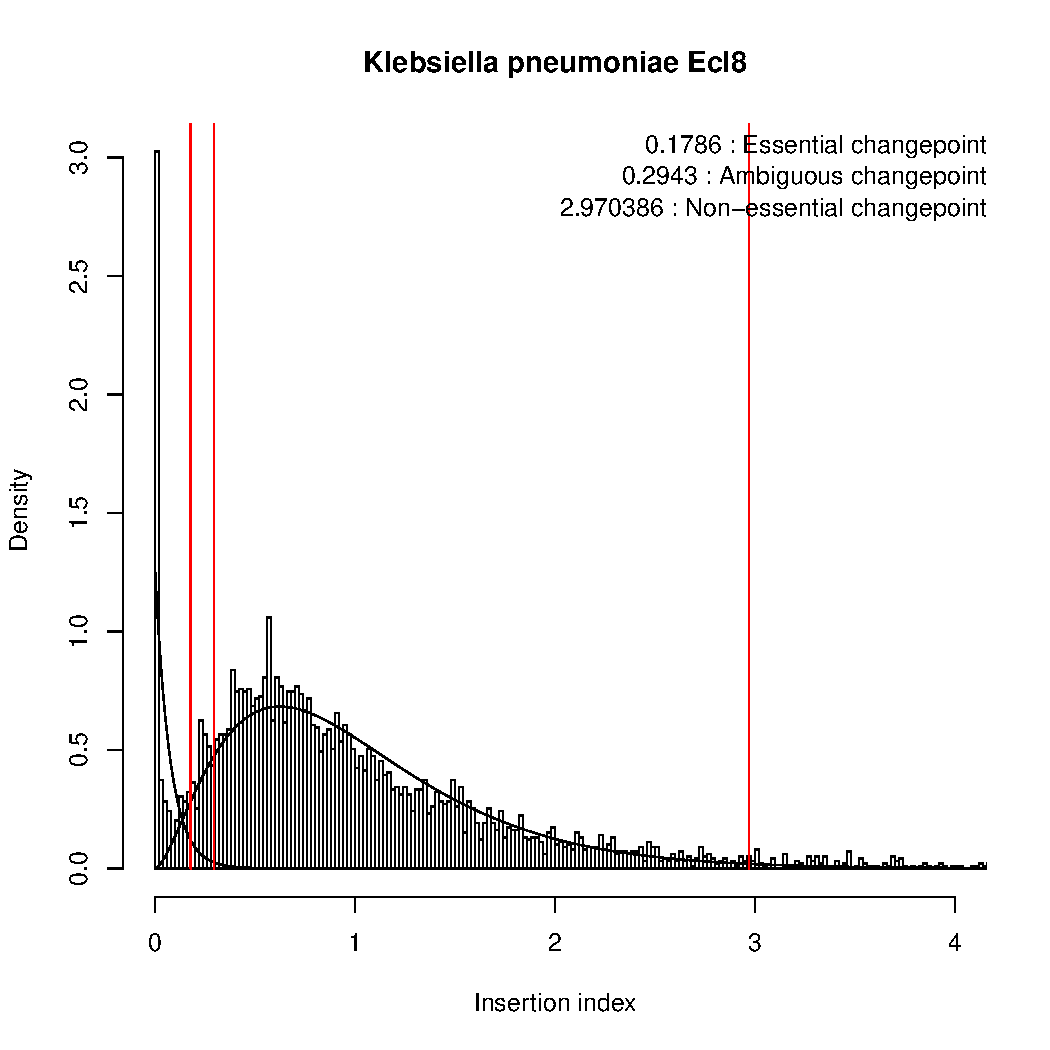
\includegraphics[scale=0.2, page=1]{lars-reads.pdf}
\includegraphics[scale=0.2, page=2]{lars-reads.pdf}
\includegraphics[scale=0.2, page=3]{lars-reads.pdf}\\
\includegraphics[scale=0.2, page=4]{lars-reads.pdf}
\includegraphics[scale=0.2, page=5]{lars-reads.pdf}
\includegraphics[scale=0.2, page=6]{lars-reads.pdf}\\
\includegraphics[scale=0.2, page=7]{lars-reads.pdf}
\includegraphics[scale=0.2, page=8]{lars-reads.pdf}
\includegraphics[scale=0.2, page=9]{lars-reads.pdf}\\
\includegraphics[scale=0.2, page=10]{lars-reads.pdf}
\includegraphics[scale=0.2, page=11]{lars-reads.pdf}
\includegraphics[scale=0.2, page=12]{lars-reads.pdf}
\caption{$ii=\frac{\frac{reads(gene)}{length(gene)}}{\frac{reads(genome)}{length(genome)}}$\newline
\textbf{Method:} Lars' method \newline
\textbf{trimming:} 5 prime site: 5\%, 3 prime site: 10\%\newline
\textbf{plot manipulations:} Lars' manipulations\newline
\textbf{Number of essential genes:}\newline
Klebsiella pneumoniae Ecl8: 322 \newline
Escherichia coli ETEC CS17: 528 \newline
Enterobacter: 351 \newline
Klebsiella pneumoniae RH201207: 387 \newline
Escherichia coli ETEC H10407: 429 \newline
Escherichia coli UPEC: 354 \newline
Citrobacter: 330 \newline
Salmonella enteritidis: 285 \newline
Salmonella typhimurium SL1344: 416 \newline
Salmonella typhimurium D23580: 333 \newline
Salmonella typhimurium A130: 357 \newline
Salmonella typhi: 361}
\end{figure}

\begin{figure}
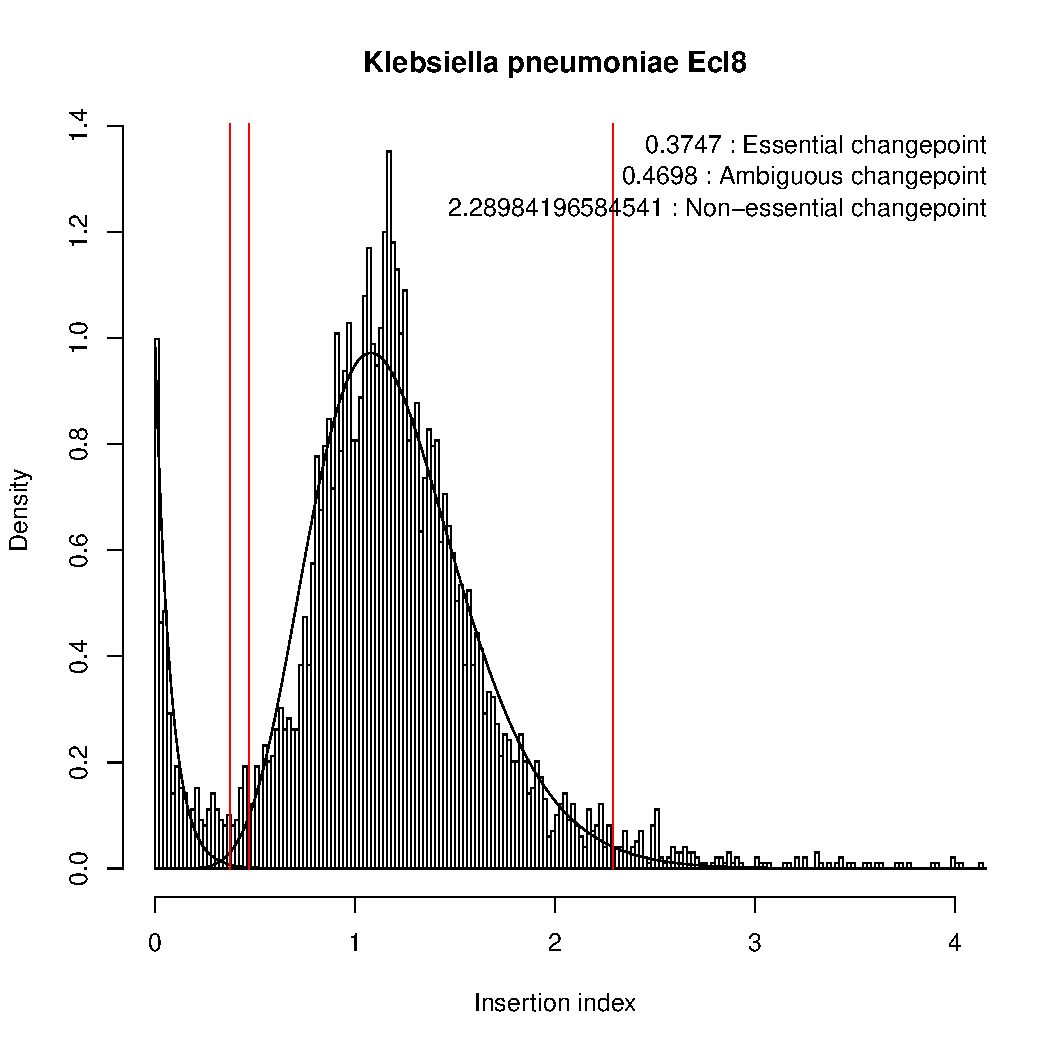
\includegraphics[scale=0.2, page=1]{results-normalised.pdf}
\includegraphics[scale=0.2, page=2]{results-normalised.pdf}
\includegraphics[scale=0.2, page=3]{results-normalised.pdf}\\
\includegraphics[scale=0.2, page=4]{results-normalised.pdf}
\includegraphics[scale=0.2, page=5]{results-normalised.pdf}
\includegraphics[scale=0.2, page=6]{results-normalised.pdf}\\
\includegraphics[scale=0.2, page=7]{results-normalised.pdf}
\includegraphics[scale=0.2, page=8]{results-normalised.pdf}
\includegraphics[scale=0.2, page=9]{results-normalised.pdf}\\
\includegraphics[scale=0.2, page=10]{results-normalised.pdf}
\includegraphics[scale=0.2, page=11]{results-normalised.pdf}
\includegraphics[scale=0.2, page=12]{results-normalised.pdf}
\caption{$ii=\frac{\frac{insertion(gene)}{length(gene)}}{\frac{insertionss(genome)}{length(genome)}}$\newline
\textbf{Method:} Lars' method \newline
\textbf{trimming:} 5 prime site: 5\%, 3 prime site: 10\%\newline
\textbf{plot manipulations:} Lars' manipulations + normalised ii for GC bias and gene location\newline
\textbf{Number of essential genes:}\newline
Klebsiella pneumoniae Ecl8: 399 \newline
Escherichia coli ETEC CS17: 648 \newline
Enterobacter: 389 \newline
Klebsiella pneumoniae RH201207: 433 \newline
Escherichia coli ETEC H10407: 480 \newline
Escherichia coli UPEC: 411 \newline
Citrobacter: 358 \newline
Salmonella enteritidis: 354 \newline
Salmonella typhimurium SL1344: 453 \newline
Salmonella typhimurium D23580: 384 \newline
Salmonella typhimurium A130: 385 \newline
Salmonella typhi: 380}
\end{figure}

\begin{figure}
\includegraphics[scale=0.2, page=1]{results-normalised-distance.pdf}
\includegraphics[scale=0.2, page=2]{results-normalised-distance.pdf}
\includegraphics[scale=0.2, page=3]{results-normalised-distance.pdf}\\
\includegraphics[scale=0.2, page=4]{results-normalised-distance.pdf}
\includegraphics[scale=0.2, page=5]{results-normalised-distance.pdf}
\includegraphics[scale=0.2, page=6]{results-normalised-distance.pdf}\\
\includegraphics[scale=0.2, page=7]{results-normalised-distance.pdf}
\includegraphics[scale=0.2, page=8]{results-normalised-distance.pdf}
\includegraphics[scale=0.2, page=9]{results-normalised-distance.pdf}\\
\includegraphics[scale=0.2, page=10]{results-normalised-distance.pdf}
\includegraphics[scale=0.2, page=11]{results-normalised-distance.pdf}
\includegraphics[scale=0.2, page=12]{results-normalised-distance.pdf}
\caption{$ii=\frac{\frac{insertion(gene)}{length(gene)}}{\frac{insertionss(genome)}{length(genome)}}$\newline
\textbf{Method:} Lars' method \newline
\textbf{trimming:} 5 prime site: 5\%, 3 prime site: 10\%\newline
\textbf{plot manipulations:} Lars' manipulations + normalised ii for gene location\newline
\textbf{Number of essential genes:}\newline
Klebsiella pneumoniae Ecl8: 351 \newline
Escherichia coli ETEC CS17: 555 \newline
Enterobacter: 347 \newline
Klebsiella pneumoniae RH201207: 400 \newline
Escherichia coli ETEC H10407: 432 \newline
Escherichia coli UPEC: 353 \newline
Citrobacter: 325 \newline
Salmonella enteritidis: 317 \newline
Salmonella typhimurium SL1344: 427 \newline
Salmonella typhimurium D23580: 358 \newline
Salmonella typhimurium A130: 354 \newline
Salmonella typhi: 334}
\end{figure}
\end{document}